\documentclass[12pt]{article}
\usepackage{tikz}
\usepackage{geometry}

\usetikzlibrary{mindmap}

\author{ supercentinel }
%2019-01-01
\geometry{landscape, margin=1cm}

\begin{document}
\begin{center}
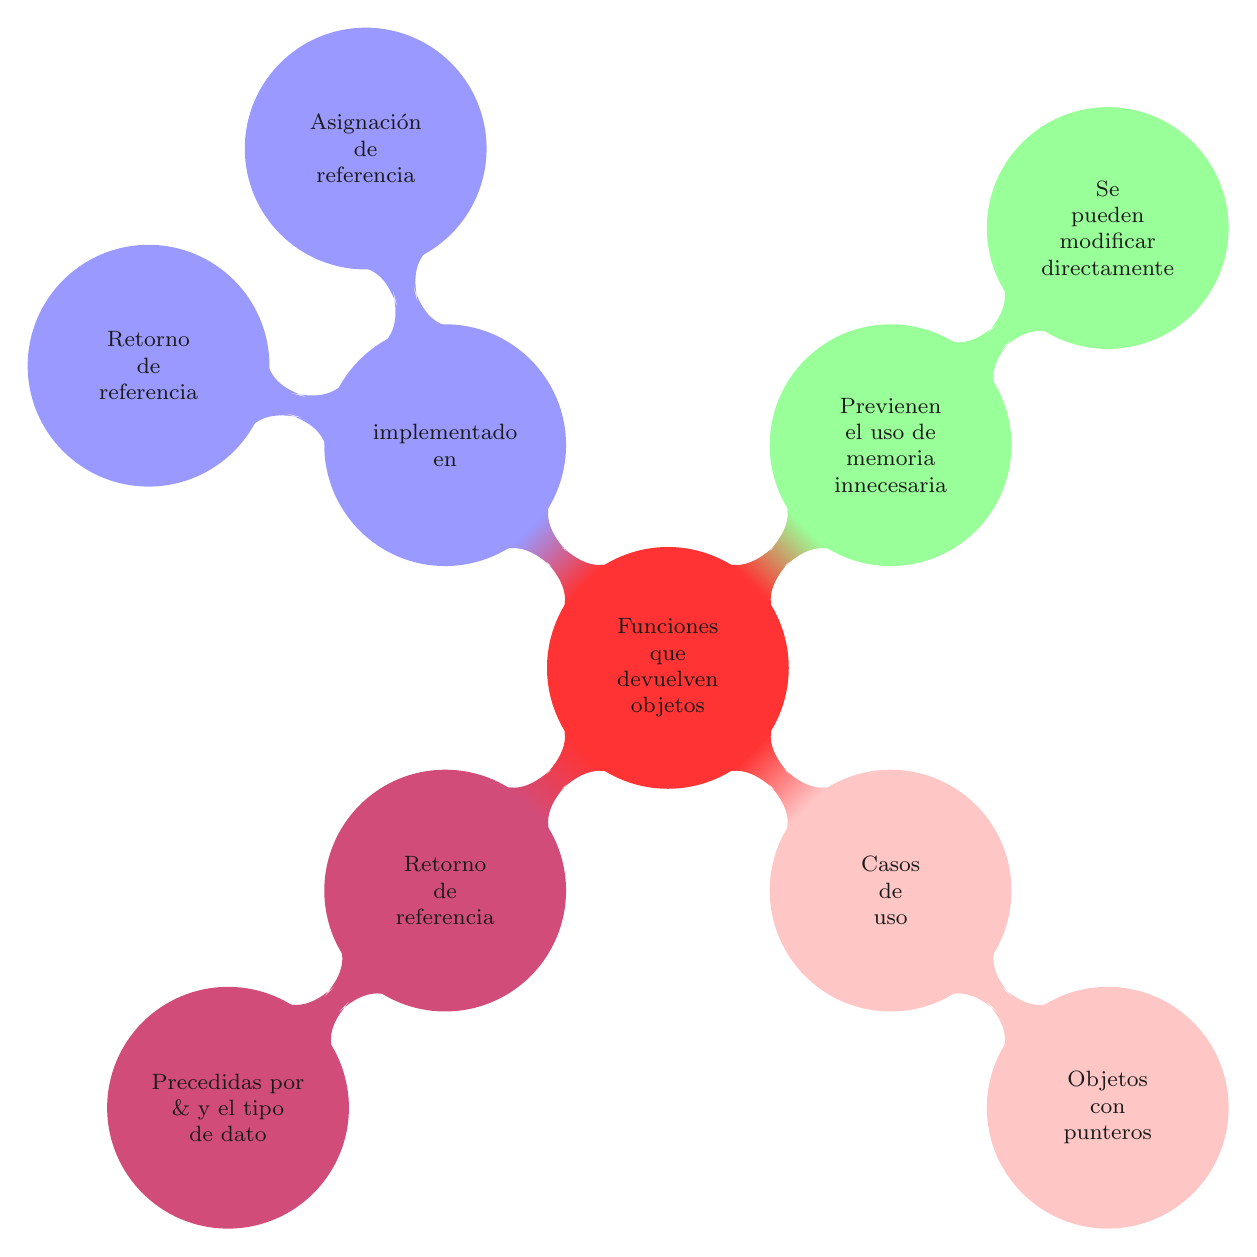
\begin{tikzpicture}[small mindmap, grow cyclic, every node/.style=concept, concept color=red!80, text=black!90, minimum size=3.0cm,
    level 1/.style={level distance=4.5cm,sibling angle=360/4},
    level 1/.style={level distance=4.0cm,sibling angle=360/4},
    level 2/.style={level distance=3.9cm,sibling angle=60},
    level 3/.style={level distance=3.5cm,sibling angle=60},
    ]
    \node{ Funciones\\que\\devuelven\\objetos }
    child[concept color=purple!70] { node { Retorno\\de\\referencia }
        child { node { Precedidas por\\\& y el tipo de dato} }
    }
    child[concept color=pink!90] { node { Casos\\de\\uso }
        child { node { Objetos\\con\\punteros } }
    }
    child[concept color=green!40] { node { Previenen\\el uso de\\memoria\\innecesaria }
        child { node { Se\\pueden\\modificar\\directamente } }
    }
    child[concept color=blue!40] { node { implementado\\en }
        child { node { Asignación\\de\\referencia }}
        child { node { Retorno\\de\\referencia }}
    }
    ;
\end{tikzpicture}
\end{center}
\end{document}
